%!TEX root = guide2.0.tex


\section*{An example statistical model}
Consider the following dataset, which is a time series of recorded coal mining disasters in the UK from 1851 to 1962.
\begin{center}
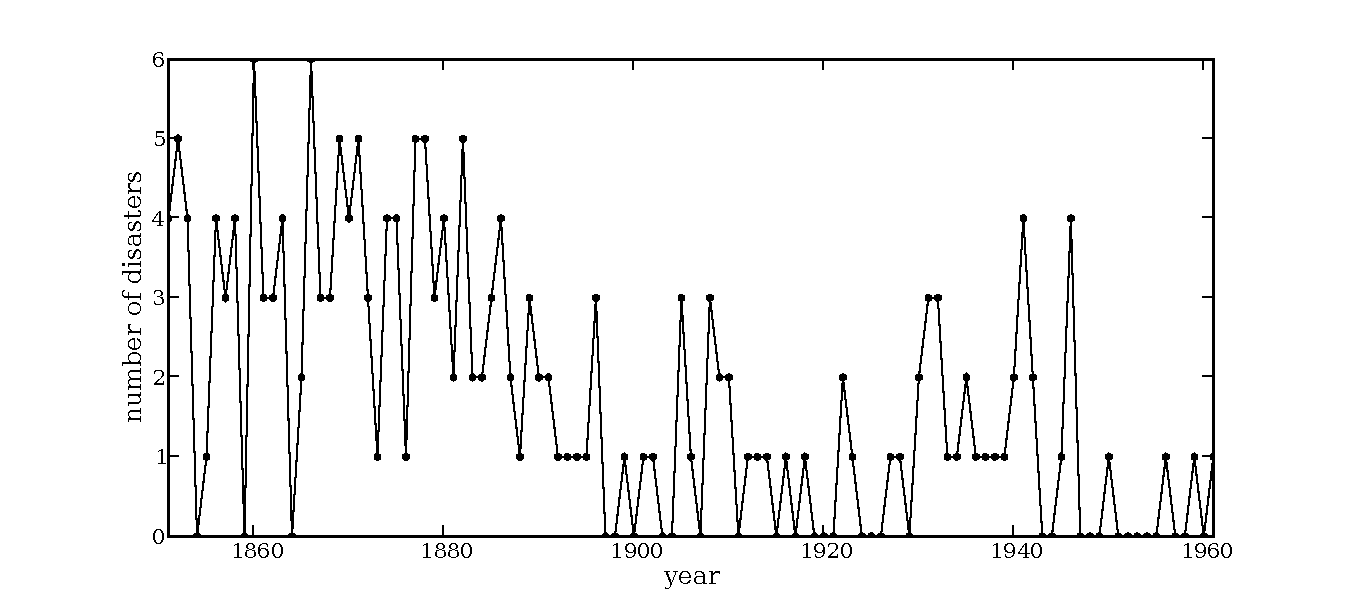
\epsfig{file=disasterts.pdf, width=15cm}
\end{center}
Occurrences of disasters in the time series is thought to be derived from a Poisson process with a large rate parameter in the early part of the time series, and from one with a smaller rate in the later part. We are interested in locating the change point in the series, which perhaps is related to changes in mining safety regulations.

We represent our conceptual model formally as a statistical model:
\begin{equation}
    \begin{array}{ccc}
        (D_t | s, e, l) \sim \textup{Poisson}\left(r_t\right), & r_t=\left\{\begin{array}{ll}
            e & t< s\\ l & t\ge s
            \end{array}\right.,&t\in[t_l,t_h]\\
        s\sim \textup{Uniform}(t_l, t_h)\\
        e\sim \textup{Exponential}(r_e)\\
        l\sim \textup{Exponential}(r_l)        
    \end{array}
    \label{disastermodel} 
\end{equation}
The symbols have the following meanings:
\begin{description}
    \item[$D_t$:] The number of disasters in year $t$.
    \item[$r_t$:] The rate parameter of the Poisson distribution of disasters in year $t$.
    \item[$s$:] The year in which the rate parameter changes.
    \item[$e$:] The rate parameter before the switchpoint $s$.
    \item[$l$:] The rate parameter after the switchpoint.
    \item[$t_l$ and $t_h$:] The lower and upper boundaries of time $t$.
    \item[$r_e$ and $r_l$:] Prior parameters.
\end{description}
Because we have defined $D$ by its dependence on $s$, $e$ and $l$, the latter three are known as the `parents' of $D$ and $D$ is called their `child'. Similarly, the parents of $s$ are $t_l$ and $t_h$, and $s$ is the child of $t_l$ and $t_h$.

\section*{Conditionally stochastic and conditionally deterministic variables}

At the model-specification stage (before the data have been observed), $D$, $s$, $e$, $r$ and $l$ are all random variables. Under the Bayesian interpretation of probability, `random' variables have not necessarily arisen from a physical random process. `Random' only means that we are unsure of their values. Random variables are represented in PyMC by class \texttt{Variable}, which has subclasses \texttt{Stochastic} and \texttt{Deterministic}.

There is a difference between $r$ and the other variables: if we knew the values of $r$'s parents, we could compute the value of $r$ with no uncertainty. This variable is defined by a mathematical function which returns its value given values for its parents. The \texttt{Deterministic} class represents such variables. This nomenclature is a bit confusing, because these objects usually represent random variables; if the parents of $r$ are random, $r$ is random also. If verbosity were not a problem, the best name for this class would probably be \texttt{DeterminedByValuesOfParents}.

On the other hand, even given values for the parents of $s$ we would still be uncertain of $s$'s value, and similarly for $D$, $e$ and $l$. These variables are defined by probability distributions that express how plausible their candidate values are given values for their parents. The \texttt{Stochastic} class represents these variables. The best name for these objects would probably be \texttt{RandomEvenGivenValuesOfParents}.

We can represent model \ref{disastermodel} in a file called \module{DisasterModel.py} as follows. First, we import the PyMC and NumPy namespaces and enter the actual data values into an array:
\begin{verbatim}
   # DisasterModel.py
   
   from pymc import *
   from numpy import *

   D_array =   array([ 4, 5, 4, 0, 1, 4, 3, 4, 0, 6, 3, 3, 4, 0, 2, 6,
                       3, 3, 5, 4, 5, 3, 1, 4, 4, 1, 5, 5, 3, 4, 2, 5,
                       2, 2, 3, 4, 2, 1, 3, 2, 2, 1, 1, 1, 1, 3, 0, 0,
                       1, 0, 1, 1, 0, 0, 3, 1, 0, 3, 2, 2, 0, 1, 1, 1,
                       0, 1, 0, 1, 0, 0, 0, 2, 1, 0, 0, 0, 1, 1, 0, 2,
                       3, 3, 1, 1, 2, 1, 1, 1, 1, 2, 4, 2, 0, 0, 1, 4,
                       0, 0, 0, 1, 0, 0, 0, 0, 0, 1, 0, 0, 1, 0, 1])
\end{verbatim} 
Next, we create the switchpoint variable $s$:
\begin{verbatim}
   s = DiscreteUniform('s', lower=0, upper=110)   
\end{verbatim}
\texttt{DiscreteUniform} is a subclass of \texttt{Stochastic} that represents uniformly-distributed discrete variables. Now we create the exponentially-distributed variables $e$ and $l$:
\begin{verbatim}
   e = Exponential('e', beta=1)
   l = Exponential('l', beta=1)   
\end{verbatim}
Now, we define the variable $r$, which selects the early rate $e$ for times before $s$ and the late rate $l$ for times after $s$. We create $r$ using the \texttt{deterministic} decorator, which converts the ordinary Python function $r$ into a \texttt{Deterministic} object.
\begin{verbatim}
   @deterministic
   def r(s=s, e=e, l=l):
      out = np.empty(110)
      out[:s] = e
      out[s:] = l
      return out
\end{verbatim}
The last step is to define the number of disasters $D$. This is done the same way as for stochastic variables, except that we set the init argument \texttt{isdata} to \texttt{True}. This tells PyMC that this object has a fixed value and does not need to be sampled:
\begin{verbatim}
   D = Poisson('D', mu=r, value=D_array, isdata=True)
\end{verbatim}

\subsection*{Why are data and unknown variables represented by the same object?}
Since it's represented by a \texttt{Stochastic} object, $D$ is defined by its dependence on its parents $s$, $e$ and $l$ even though its value is fixed. This isn't just a quirk of PyMC's syntax; Bayesian hierarchical notation itself makes no distinction between random variables and data. The reason is simple: to use Bayes' theorem to compute the posterior $p(e,s,l|D)$ of model \ref{disastermodel}, we need to use the likelihood $p(D|e,s,l)$. Even though $D$'s value is known and fixed, we need to formally assign it a probability distribution as if it were a random variable.

This point can be counterintuitive at first, as many peoples' instinct is to regard data as fixed a priori and unknown variables as dependent on the data. One way to understand is to think of statistical models like (\ref{disastermodel}) as predictive models for data, or as models of the processes that gave rise to data. Before observing the value of $D$, we could have sampled from its prior predictive distribution $p(D)$ (\emph{i.e.} the marginal distribution of the data) as follows:
\begin{enumerate}
    \item Sample $e$, $s$ and $l$ from their priors.
    \item Sample $D$ conditional on these values.
\end{enumerate}
Even after we observe the value of $D$, we need to use this process model to make inferences about $e$, $s$ and $l$; it's the only information we have about how the variables are related.

\medskip
To look at the issue another way, we could, in principle, have written a model equivalent to (\ref{disastermodel}) in such a way that $D$ depended on nothing and everything else depended on $D$, for example
\begin{eqnarray*}
    s|e,l,D\sim\cdot\\
    e|l,D\sim\cdot\\
    l|D\sim\cdot\\
    D=D_*
\end{eqnarray*}

This would have felt more natural in some ways, because we would have the unknown stochastic variables depending on the data. However, if we could write down that model using standard distributions we could trivially compute and sample from the posterior,
\begin{eqnarray*}
    p(s,e,l|D) = p(s|e, l, D) p(e|l, D) p(l|D),
\end{eqnarray*}
and we would have no use for MCMC or any other fitting method. Bayesian methods, and statistics in general, are needed when it's feasible to write down the data's dependence on the unknown variables but not vice versa.

% ITS MORE THAN THIS, ISNT IT? THE REASON THAT THE ABOVE IS NOT INTERESTING IS THAT WE CANNOT TYPICALLY
% GET THESE VALUES -- THEY ARE EXACTLY THE POSTERIORS THAT ARE UNKNOWN (CANNOT CALCULATE THEM ANALYTICALLY)

\section*{Parents and children}

We have created a PyMC probability model: a linked collection of variables. To see the nature of the links, import or run \texttt{DisasterModel.py} and examine $s$'s \texttt{parents} attribute from the Python prompt:
\begin{verbatim}
   In [2]: s.parents
   Out[2]: {'lower': 0, 'upper': 110}
\end{verbatim}
The \texttt{parents} dictionary shows us the distributional parameters of $s$. Now try examining $D$'s parents:
\begin{verbatim}
   In [3]: D.parents
   Out[3]: {'mu': <pymc.PyMCObjects.Deterministic 'r' at 0x3e51a70>}
\end{verbatim}
We are using $r$ as a distributional parameter of $D$, so $r$ is $D$'s parent. $D$ labels $r$ as \texttt{mu}, meaning it plays the role of the rate parameter in $D$'s Poisson distribution. Now examine $r$'s \texttt{children} attribute:
\begin{verbatim}
   In [3]: r.children
   Out[3]: set([<pymc.distributions.Poisson 'D' at 0x3e51290>])
\end{verbatim}
Because $D$ considers $r$ its parent, $r$ considers $D$ its child. Unlike \texttt{parents}, \texttt{children} is a set; variables do not associate their children with any particular distributional role. Try examining the \texttt{parents} and \texttt{children} attributes of the other parameters in the model.

\section*{Variables' values and log-probabilities}
All PyMC variables have an attribute called \texttt{value}. Try examining $D$'s value, and you'll see the initial value we provided for it:
\begin{verbatim}
   In [4]: D.value
   Out[4]: 
   array([4, 5, 4, 0, 1, 4, 3, 4, 0, 6, 3, 3, 4, 0, 2, 6, 3, 3, 5, 4, 5, 3, 1,
          4, 4, 1, 5, 5, 3, 4, 2, 5, 2, 2, 3, 4, 2, 1, 3, 2, 2, 1, 1, 1, 1, 3,
          0, 0, 1, 0, 1, 1, 0, 0, 3, 1, 0, 3, 2, 2, 0, 1, 1, 1, 0, 1, 0, 1, 0,
          0, 0, 2, 1, 0, 0, 0, 1, 1, 0, 2, 3, 3, 1, 1, 2, 1, 1, 1, 1, 2, 4, 2,
          0, 0, 1, 4, 0, 0, 0, 1, 0, 0, 0, 0, 0, 1, 0, 0, 1, 0, 1])
\end{verbatim}
If you check $e$'s, $s$'s and $l$'s values, you'll see random initial values generated by PyMC (yours will be different from the following):
\begin{verbatim}
   In [5]: s.value
   Out[5]: 44

   In [6]: e.value
   Out[6]: 0.33464706250079584

   In [7]: l.value
   Out[7]: 2.6491936762267811
\end{verbatim}
If you check $r$'s value, you'll see an array whose first $s$ elements are \texttt{e.value}, and whose remaining elements are \texttt{l.value}:
\begin{verbatim}
   In [8]: r.value
   Out[8]: 
   array([ 0.33464706,  0.33464706,  0.33464706,  0.33464706,  0.33464706,
           0.33464706,  0.33464706,  0.33464706,  0.33464706,  0.33464706,
           0.33464706,  0.33464706,  0.33464706,  0.33464706,  0.33464706,
           0.33464706,  0.33464706,  0.33464706,  0.33464706,  0.33464706,
           0.33464706,  0.33464706,  0.33464706,  0.33464706,  0.33464706,
           0.33464706,  0.33464706,  0.33464706,  0.33464706,  0.33464706,
           0.33464706,  0.33464706,  0.33464706,  0.33464706,  0.33464706,
           0.33464706,  0.33464706,  0.33464706,  0.33464706,  0.33464706,
           0.33464706,  0.33464706,  0.33464706,  0.33464706,  2.64919368,
           2.64919368,  2.64919368,  2.64919368,  2.64919368,  2.64919368,
           2.64919368,  2.64919368,  2.64919368,  2.64919368,  2.64919368,
           2.64919368,  2.64919368,  2.64919368,  2.64919368,  2.64919368,
           2.64919368,  2.64919368,  2.64919368,  2.64919368,  2.64919368,
           2.64919368,  2.64919368,  2.64919368,  2.64919368,  2.64919368,
           2.64919368,  2.64919368,  2.64919368,  2.64919368,  2.64919368,
           2.64919368,  2.64919368,  2.64919368,  2.64919368,  2.64919368,
           2.64919368,  2.64919368,  2.64919368,  2.64919368,  2.64919368,
           2.64919368,  2.64919368,  2.64919368,  2.64919368,  2.64919368,
           2.64919368,  2.64919368,  2.64919368,  2.64919368,  2.64919368,
           2.64919368,  2.64919368,  2.64919368,  2.64919368,  2.64919368,
           2.64919368,  2.64919368,  2.64919368,  2.64919368,  2.64919368,
           2.64919368,  2.64919368,  2.64919368,  2.64919368,  2.64919368])
\end{verbatim}
To compute its value, $r$ calls the funtion we used to create it, passing in the values of its parents.

Stochastic objects can evaluate their probability mass or density functions at their current values given the values of their parents. The log of a stochastic object's probability mass or density can be accessed via the \texttt{logp} attribute. For vector-valued variables like $D$, the \texttt{logp} attribute returns the log of the joint probability or density of all elements of the value. Try examining $s$'s and $D$'s log-probabilities and $e$'s and $l$'s log-densities:
\begin{verbatim}
   In [9]: s.logp
   Out[9]: -4.7095302013123339

   In [10]: D.logp
   Out[10]: -1080.5149888046033

   In [11]: e.logp
   Out[11]: -0.33464706250079584

   In [12]: l.logp
   Out[12]: -2.6491936762267811
\end{verbatim}
Stochastic objects need to call an internal function to compute their \texttt{logp} attributes, as $r$ needed to call an internal function to compute its value. Just as we created $r$ by decorating a function that computes its value, it's possible to create custom \texttt{Stochastic} objects by decorating functions that compute their log-probabilities or densities (see chapter \ref{chap:modelbuilding}). 

\subsection*{Using \texttt{Variables} as parents of \texttt{Variables}}

Let's take a closer look at our definition of $r$:
\begin{verbatim}
   @deterministic
   def r(s=s, e=e, l=l):
      out = np.empty(111)
      out[:s] = e
      out[s:] = l
      return out
\end{verbatim}
The arguments are \texttt{Stochastic} objects, not numbers. Why aren't errors raised when we attempt to slice array \texttt{out} up to a \texttt{Stochastic} object?

Whenever a variable is used as a parent for a child variable, it is replaced with its \texttt{value} attribute when the child's value or log-probability is computed. When $r$'s value is recomputed, \texttt{s.value} is passed to the function as argument \texttt{s}. To see the values of the parents of $r$ all together, look at \texttt{r.parents.value}.

\section*{Fitting the model with MCMC}

PyMC provides several objects that fit probability models (linked collections of variables) like ours. The primary such object, \texttt{MCMC}, fits models with the Markov chain Monte Carlo algorithm. See chapter \ref{chap:MCMC} for an introduction to the algorithm itself. To create an \texttt{MCMC} object to handle our model, add the following line to \module{DisasterModel.py}:
\begin{verbatim}
   M = MCMC([s,e,l,D])
\end{verbatim}
To actually fit the model, call the MCMC object's \texttt{isample()} method, either from \module{DisasterModel.py} or the prompt:
\begin{verbatim}
   M.isample(iter=10000, burn=1000, thin=1)
\end{verbatim}
After a few seconds, you should see that sampling has finished normally. The model has been fitted.

\subsection*{What does it mean to fit a model?}
The output of the MCMC algorithm is a `trace', or a long list of samples for each variable in the model. These traces are stored on the variables themselves and can be accessed using the \texttt{trace()} method:
\begin{verbatim}
   In [2]: s.trace()
   Out[2]: array([41, 40, 40, ..., 43, 44, 44])
\end{verbatim}
The unknown variables $s$, $e$, $l$ and $r$ will all get traces, but $D$ will not because its value has been observed and is not updated. After burn-in, the $i$'th elements of all the variables' traces can be considered a joint sample from the posterior distribution.


\subsection*{Sampling output} 
You can examine the marginal posterior of any variable by plotting a histogram of its trace:
\begin{verbatim}
   In [3]: from pylab import *
   In [3]: hist(l.trace())
   Out[3]: 
   (array([   8,   52,  565, 1624, 2563, 2105, 1292,  488,  258,   45]),
    array([ 0.52721865,  0.60788251,  0.68854637,  0.76921023,  0.84987409,
           0.93053795,  1.01120181,  1.09186567,  1.17252953,  1.25319339]),
    <a list of 10 Patch objects>)
\end{verbatim}
You should see something like this:
\begin{center}
   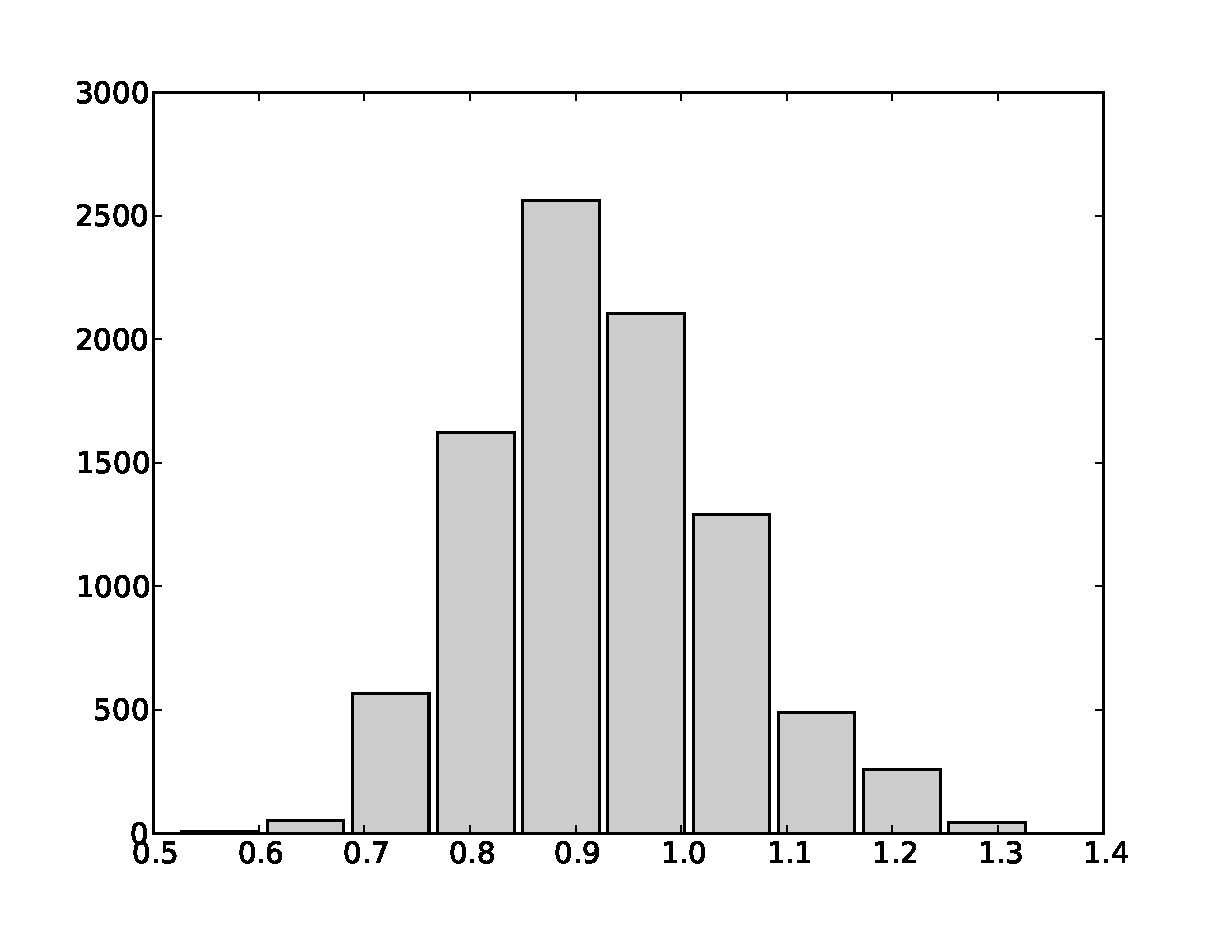
\epsfig{file=ltrace.pdf, width=10cm}
\end{center}

To see plots of all the scalar variables, simply type 
\begin{verbatim}
   In [4]: M.plot()
\end{verbatim}
You will see several figures like the following:
\begin{center}
   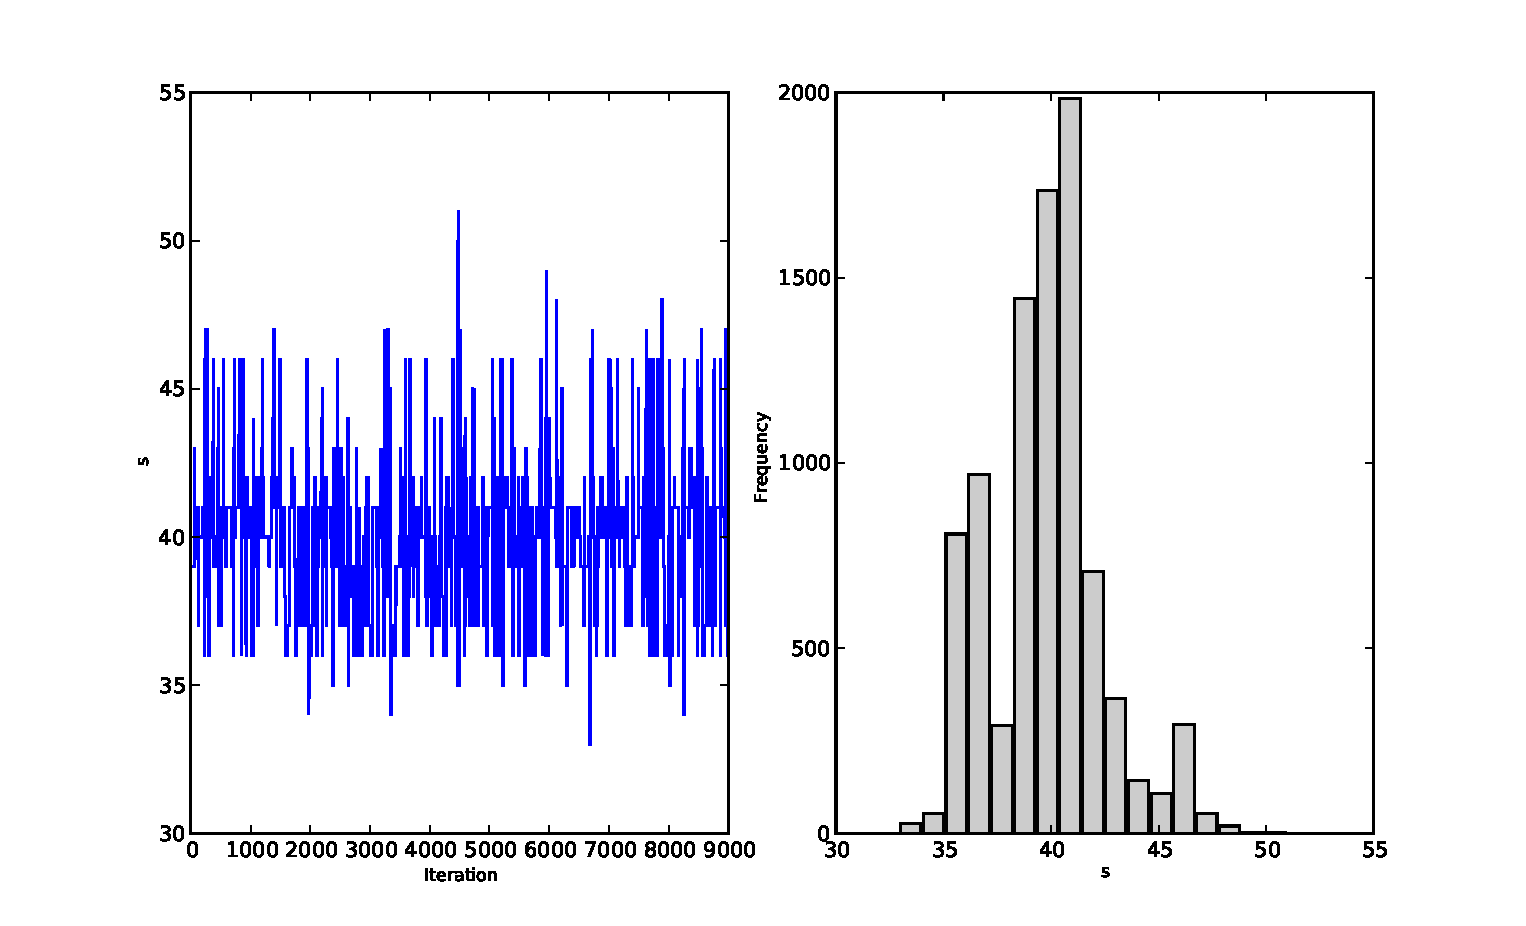
\epsfig{file=spost.pdf, width=15cm}
\end{center}
The left-hand pane of this figure shows the actual trace of $s$, and the right-hand pane shows a histogram of the trace. The left-hand pane is useful for evaluating and diagnosing the algorithm's performance [\textbf{ref}]. If the trace looks good, the right-hand pane is useful for visualizing the posterior. The posterior of $s$ seems to be bimodal, which is interesting.

For a non-graphical summary of the posterior, simply call \texttt{M.stats()}.


\section*{Fine-tuning the MCMC algorithm} 

MCMC objects handle individual variables via `step methods'. By default, step methods are automatically assigned to variables by PyMC. To see which step methods $M$ is using, look at its \texttt{step_method_dict} attribute:
\begin{verbatim}
   In [5]: M.step_method_dict[s]
   Out[5]: [<pymc.StepMethods.DiscreteMetropolis object at 0x3e8cb50>]
   
   In [8]: M.step_method_dict[e]
   Out[8]: [<pymc.StepMethods.Metropolis object at 0x3e8cbb0>]

   In [9]: M.step_method_dict[l]
   Out[9]: [<pymc.StepMethods.Metropolis object at 0x3e8ccb0>]
\end{verbatim}
The value of \texttt{step_method_dict} corresponding to a particular variable is a list of the step methods $M$ is using to handle that variable. 

You can force $M$ to use a particular step method by calling \texttt{M.use_step_method} before telling it to sample. The following call will cause $M$ to handle $l$ with a standard \texttt{Metropolis} step method, but with proposal standard deviation equal to $2$:
\begin{verbatim}
   M.use_step_method(Metropolis, l, sig=2.)
\end{verbatim}

Another step method class, \texttt{AdaptiveMetropolis}, is better at handling highly-correlated variables. If your model mixes poorly, using \texttt{AdaptiveMetropolis} is a sensible first thing to try.

You can see all the step method classes that have been defined (including user-defined step methods) in the list \texttt{StepMethodRegistry}, which is on the PyMC namespace: 
\begin{verbatim}
   In [12]: pymc.StepMethodRegistry
   Out[12]: 
   [<class 'pymc.StepMethods.StepMethod'>,
    <class 'pymc.StepMethods.NoStepper'>,
    <class 'pymc.StepMethods.Metropolis'>,
    <class 'pymc.StepMethods.Gibbs'>,
    <class 'pymc.StepMethods.NoStepper'>,
    <class 'pymc.StepMethods.DiscreteMetropolis'>,
    <class 'pymc.StepMethods.BinaryMetropolis'>,
    <class 'pymc.StepMethods.AdaptiveMetropolis'>,
    <class 'pymc.StepMethods.IIDSStepper'>,
    <class 'pymc.GP.PyMC_objects.GPParentMetropolis'>,
    <class 'pymc.GP.PyMC_objects.GPMetropolis'>,
    <class 'pymc.GP.PyMC_objects.GPNormal'>]
\end{verbatim}
See the docstrings of the individual classes for details on how to use them.

\section*{Beyond the basics}
That's all there is to basic PyMC usage. Many more topics are covered in the reference manual (all chapters after \ref{chap:MCMC}), including:
\begin{itemize}
   \item Class \texttt{Potential}, another building block for probability models in addition to \texttt{Stochastic} and \texttt{Deterministic}
   \item Normal approximations
   \item How to use custom probability distributions
   \item The inner workings of the objects
   \item How to save traces to the disk, or stream them to the disk during sampling
   \item How to write your own step methods and fitting algorithms.
\end{itemize}
Also, be sure to check out the documentation for the Gaussian process extension, located in folder \texttt{gp} in the source directory. 

\bigskip
MCMC is a surprisingly difficult and bug-prone algorithm to implement by hand. We find PyMC makes it much easier and less stressful. PyMC also makes our work more dynamic; getting hand-coded MCMC's working used to be so much work that we were reluctant to change anything, but with PyMC changing models is a breeze. We hope it does the same for you!